\documentclass[]{beamer}

\usepackage{pdfpages}
%\setbeameroption{show notes on second screen}

\usepackage[utf8]{inputenc}
\usepackage[T1]{fontenc}
\usepackage{mathabx}
\usepackage{mathpazo}
\usepackage{eulervm}
\usepackage{natbib}
\usepackage{adjustbox}
\usepackage{booktabs}

\usepackage{colortbl}

\hypersetup{colorlinks=true, urlcolor=blue, linkcolor=white, citecolor=blue}

\usepackage{caption}
\captionsetup[figure]{labelformat=empty}% redefines the caption setup of the figures environment in the beamer class.

\usetheme{Madrid}
\definecolor{uog}{rgb}{0,.5,0}
\usecolortheme[named=uog]{structure}

%\mode<handout>{
%    \pgfpagesuselayout{4 on 1}[letterpaper] 
%    \setbeameroption{show notes}
%}


% The following code uses \AtBeginSection to place a frame with the section title (\insertsectionhead) inside a beamercolorbox.
% From https://tex.stackexchange.com/questions/178800/creating-sections-each-with-title-pages-in-beamers-slides
\AtBeginSection[]{
  \begin{frame}
  \vfill
  \centering
  \begin{beamercolorbox}[sep=8pt,center,shadow=true,rounded=true]{title}
    \usebeamerfont{title}\insertsectionhead\par%
  \end{beamercolorbox}
  \vfill
  \end{frame}
}


\title[Coconut Rhinoceros Beetle Catastrophe]{Coconut Rhinoceros Beetle Causes\\an Ecological Catastrophe on Guam}

\author{Aubrey Moore}

\institute[University of Guam]{Extension and Outreach\\College of Natural and Applied Sciences\\University of Guam}

\titlegraphic{
\includegraphics[width=2cm]{big_g2.pdf}}

\date[]{Presentation for UOG Extension Interns\\June 21, 2019}

\begin{document}

%\maketitle

\begin{frame}
	\scriptsize{Potentially Catastrophic Science!}
	\titlepage
\end{frame}

\section{Introduction}

\begin{frame}{Definition of Catastrophe}
	
\begin{itemize}
\item (colloquial) A large, often sudden, disaster
\item (mathematics) A type of bifurcation, where a system shifts between two stable states
\end{itemize}

\centering
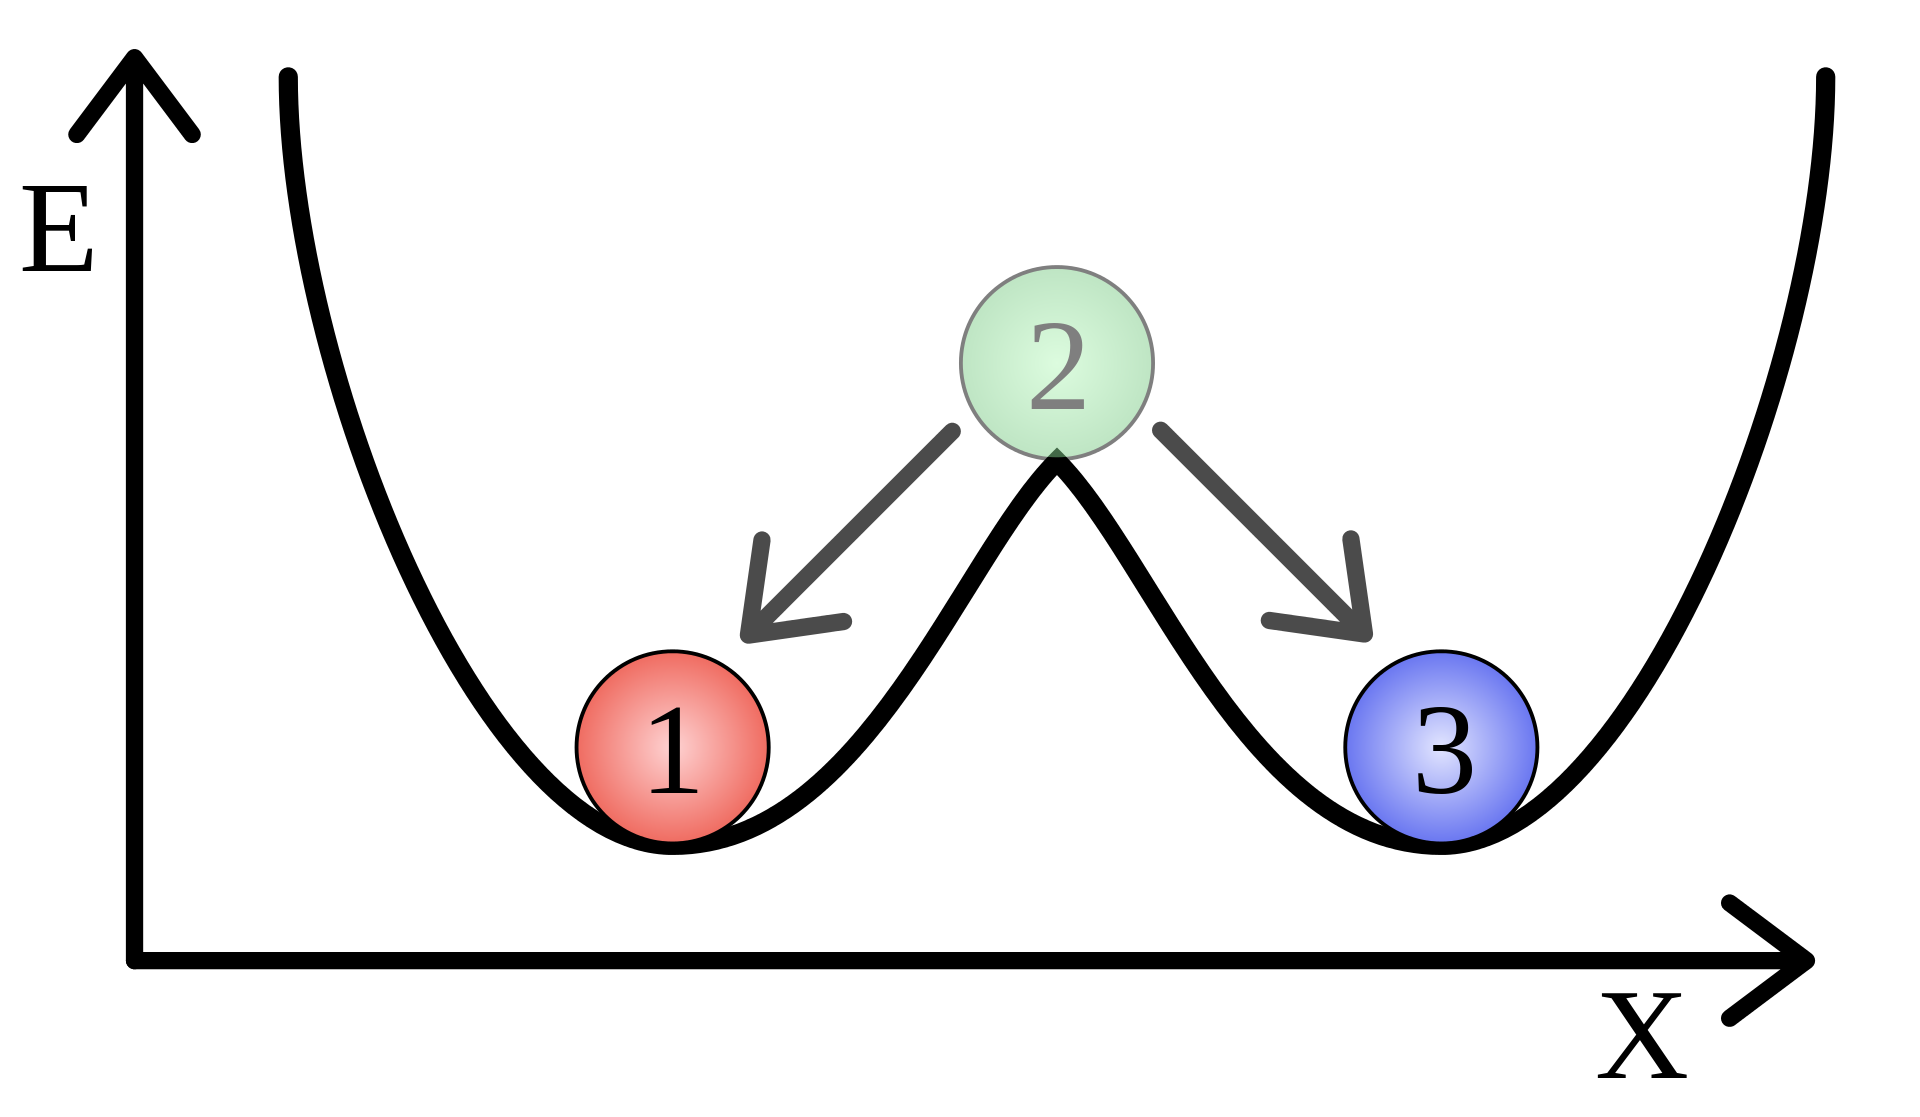
\includegraphics[width=.6\linewidth]{bistable.png}

\end{frame}







{
	\setbeamercolor{background canvas}{bg=}
	\includepdf[pages=3]{AubreyICE2016.pdf}
}

\begin{frame}{Geographic Distribution of Coconut Rhinoceros Beetle}
	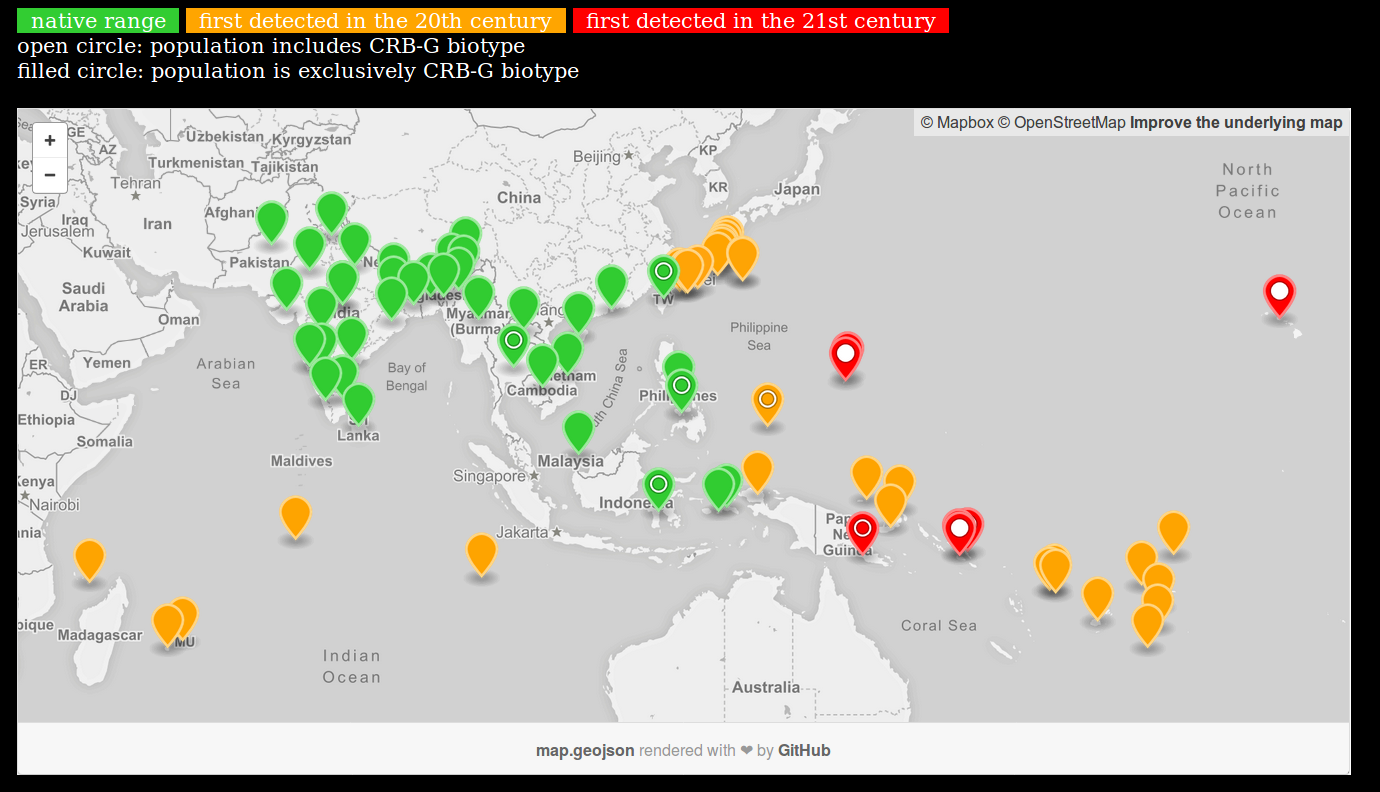
\includegraphics[width=\linewidth]{crb_map.png}
\end{frame}

{
	\setbeamercolor{background canvas}{bg=}
	\includepdf[pages=5-7]{AubreyICE2016.pdf}
}

{
	\setbeamercolor{background canvas}{bg=}
	\includepdf[pages=9-11]{CRB-RISC-MAR-2013.pdf}
}

{
	\setbeamercolor{background canvas}{bg=}
	\includepdf[pages=8-]{AubreyICE2016.pdf}
}

\section{Conclusion}

\begin{frame}{CRB is Causing a Catastrophe in the Colloquial Sense}
Guam's forests are rapidly being destroyed by invasive species. Loss of palms is part of a larger catastrophe:
\begin{itemize}
	\item Brown treesnake killed most forest birds
	\item Cycad scale has killed 90 percent of Guam's endemic cycad
	\item Little fire ant is killing many other species
\end{itemize}
\end{frame}

\begin{frame}{Dominant Trees in Guam's Forests are Threatened by Asian Cycad Scale (ACS) and Coconut Rhinoceros Beetle (CRB)}
	\begin{center}
		\begin{tabular}{llcrp{0.35in}}
			\hline
			\textbf{Threat} & \textbf{Species} & \textbf{Status} & \textbf{Tree count\footnote{Estimated number of trees with DBH greater than 5 inches.}} & \textbf{\% of total tree count}\\
			\hline
			\rowcolor{yellow}
			ACS & \textit{Cycas micronesica} & endemic & 1,571,556 & 16\% \\ 
			\rowcolor{yellow}
			CRB & \textit{Cocos nucifera} & native & 1,162,494 & 12\% \\ 
			\rowcolor{yellow}
			CRB & \textit{Heterospathe elata} & introduced & 1,075,552 & 11\% \\ 		
			\hline
			& \textit{Vitex parviflora} & introduced & 902,990 & 9\% \\ 
			& \textit{Leucaena leucocephala} & introduced & 890,217 & 9\%\\
			\hline
		\end{tabular} 
	\end{center}
	Tree census data source: J. A. Donnegon et al. 2004. Guam’s Forest Resources, 2002. Available from: \url{http://www.fs.fed.us/pnw/pubs/pnw_rb243.pdf}
	\note{
		The threat to Guam's forests by these 2 species is very serious.
		
		A tree census performed in 2002 by the US Forest Service listed Guam's endemic cycad as the most common tree. 90\% of these palnts have already been killed by ACS.
		
		The census listed coconut palm and an introduced palm as Guam's second and third most common trees. These are rapidly being killed by coconut rhinoceros beetle.
	}
\end{frame}

\begin{frame}{CRB is Causing a Catastrophe in the Mathematical Sense}

	\begin{itemize}
		\item Typhoons initiated a catastrophic switch in the state of CRB population dynamics on Guam.
		\item Prior to typhoons, CRB population levels were regulated by availability of an extrinsically generated larval food supply.
		\item After typhoons, the CRB population generates its own larval food supply by killing palms.
	\end{itemize}
\end{frame}

\end{document}
